
% \begin{figure}[H]
% 	\centering	\includegraphics[width=0.8\textwidth]{img/nombre.png}
% 	\caption{Titulo}
% 	\label{fig:etiqueta}
% \end{figure}

\par En cuanto al ruido, para verificar lo expicado anteriormente acerca de nuestra elección de ruido multiplicativo hicimos los siguientes experimentos.
Utilizamos una imagen de 100px x 100px, con $\alpha$ = 0.2, dividida en 5 celdas y con 100 emisores de rayos, y 100 rayos emitidos desde cada uno de estos. Luego, sobre esto comparamos el vector de tiempos de los rayos sin ruido contra el mismo con ruido multiplicativo y aditivo. 

\begin{figure}[H]
	\centering	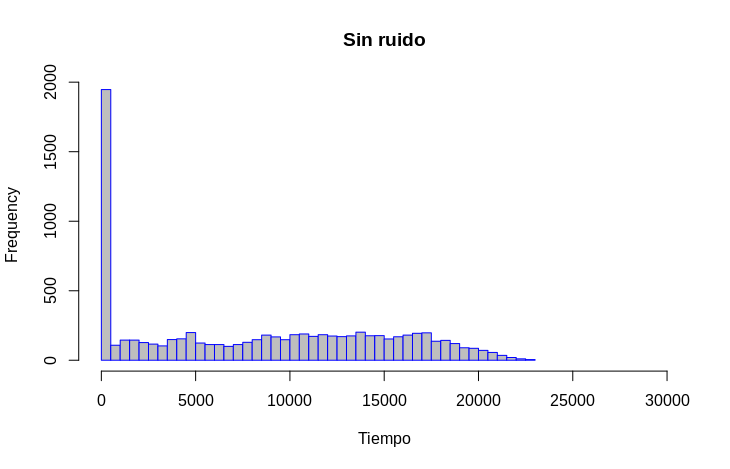
\includegraphics[width=0.7\textwidth]{img/sinRuido.png}
	\caption{Vector de tiempos de rayos sin ruido}
	\label{fig:etiqueta}
\end{figure}
\par Acá podemos observar que efectivamente, el ruido aditivo modifíca mucho más algunas partes del vector mientras que otras no se aprecian muchos cambios. En este caso el histograma de ruido aditivo sufre cambios notorios respecto del vector sin ruido, mientras que en los valores más grandes casi que no notamos se notan diferencias.

\begin{figure}[H]
	\centering	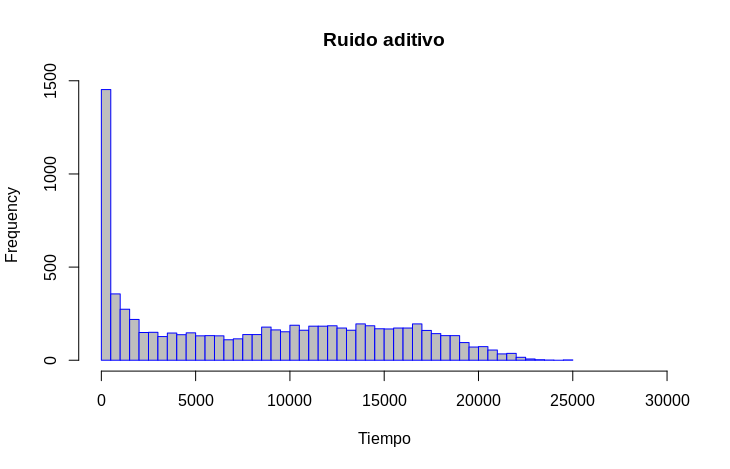
\includegraphics[width=0.7\textwidth]{img/ruidoAditivo.png}
	\caption{Vector de tiempos de rayos con ruido aditivo}
	\label{fig:etiqueta}
\end{figure}

\par En este otro caso en cambio, vemos que las diferencias entre el histograma de ruido multiplicativo y sin ruido existen pero están más uniformemente distribuídas. La única anormalidad que observamos es un incremento en los valores máximos, no obstante se trata de unos pocos casos aislados.
Esto se parece más a lo que esperabamos que hiciera nuestro ruido, por eso fue que elegimos usar este método en nuestra implementación.
\begin{figure}[H]
	\centering	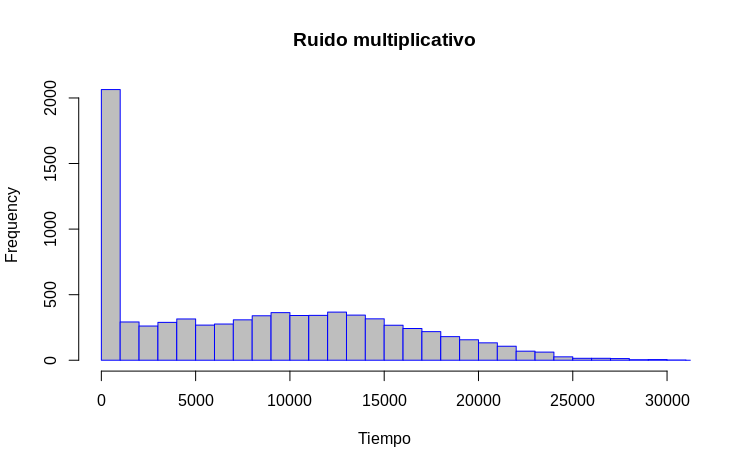
\includegraphics[width=0.7\textwidth]{img/ruidoMultiplicativo.png}
	\caption{Vector de tiempos de rayos con ruido multiplicativo}
	\label{fig:etiqueta}
\end{figure}



\begin{figure}[H]
	\centering	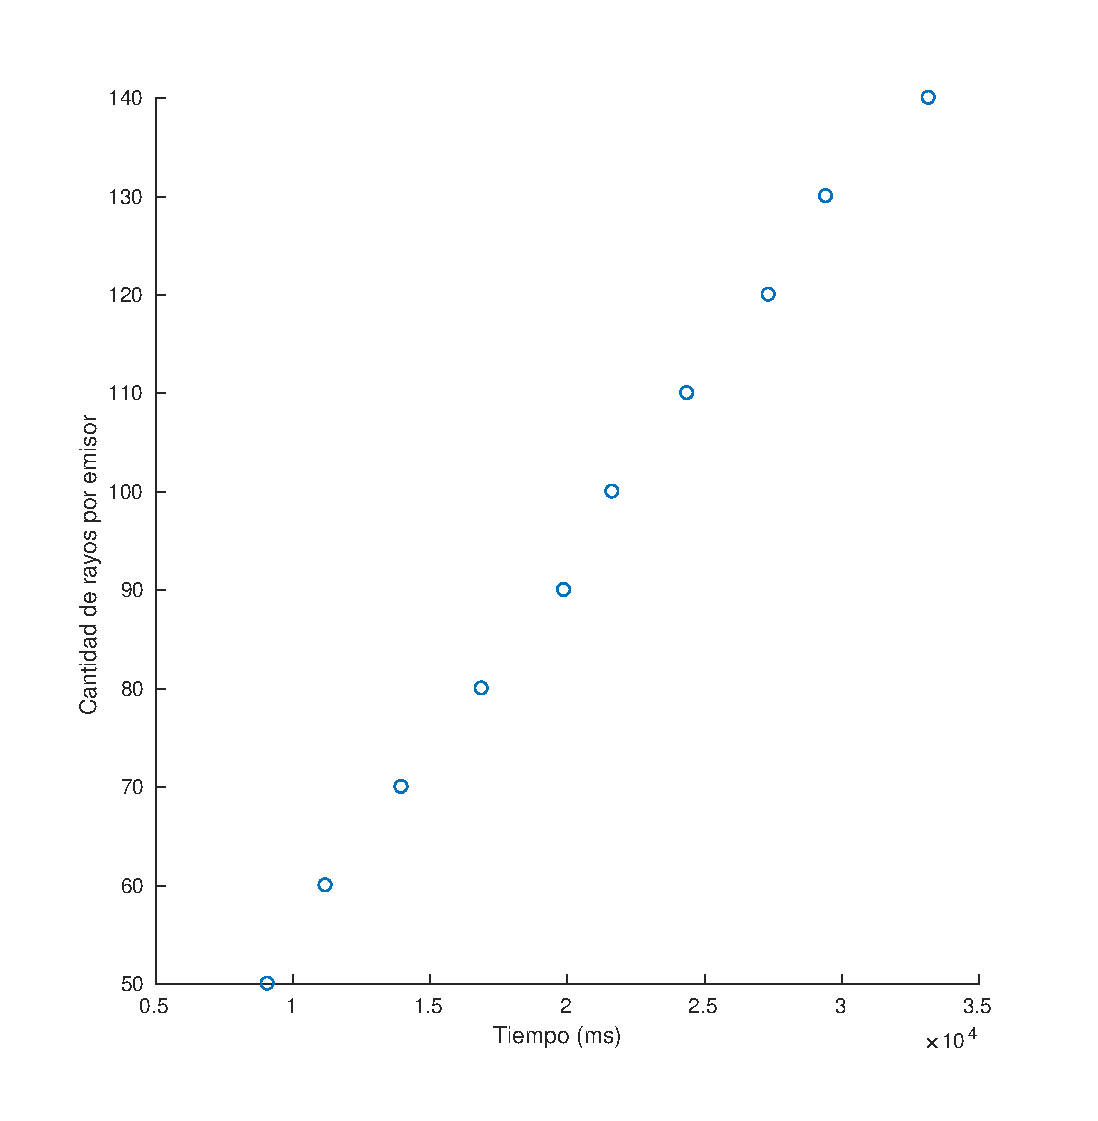
\includegraphics[width=0.7\textwidth]{img/cantrayos_tiempo}
	\caption{Tiempo en funcion de la Cantidad de rayos con granularidad, cantidad de emisores y ruido fijos}
	\label{fig:cantrayos_tiempo}
\end{figure}
\par Tal como se puede apreciar en esta imagen la cantidad de rayos que parten de cada emisor afectan de manera importante el tiempo de ejecuci\'on, lo cual consideramos que se debe a que a medida que crece la cantidad de rayos, crece el 
tamaño de las matrices con las cuales operamos por lo que la eliminaci\'on Gaussiana requiere m\'as operaciones.


\begin{figure}[H]
	\centering	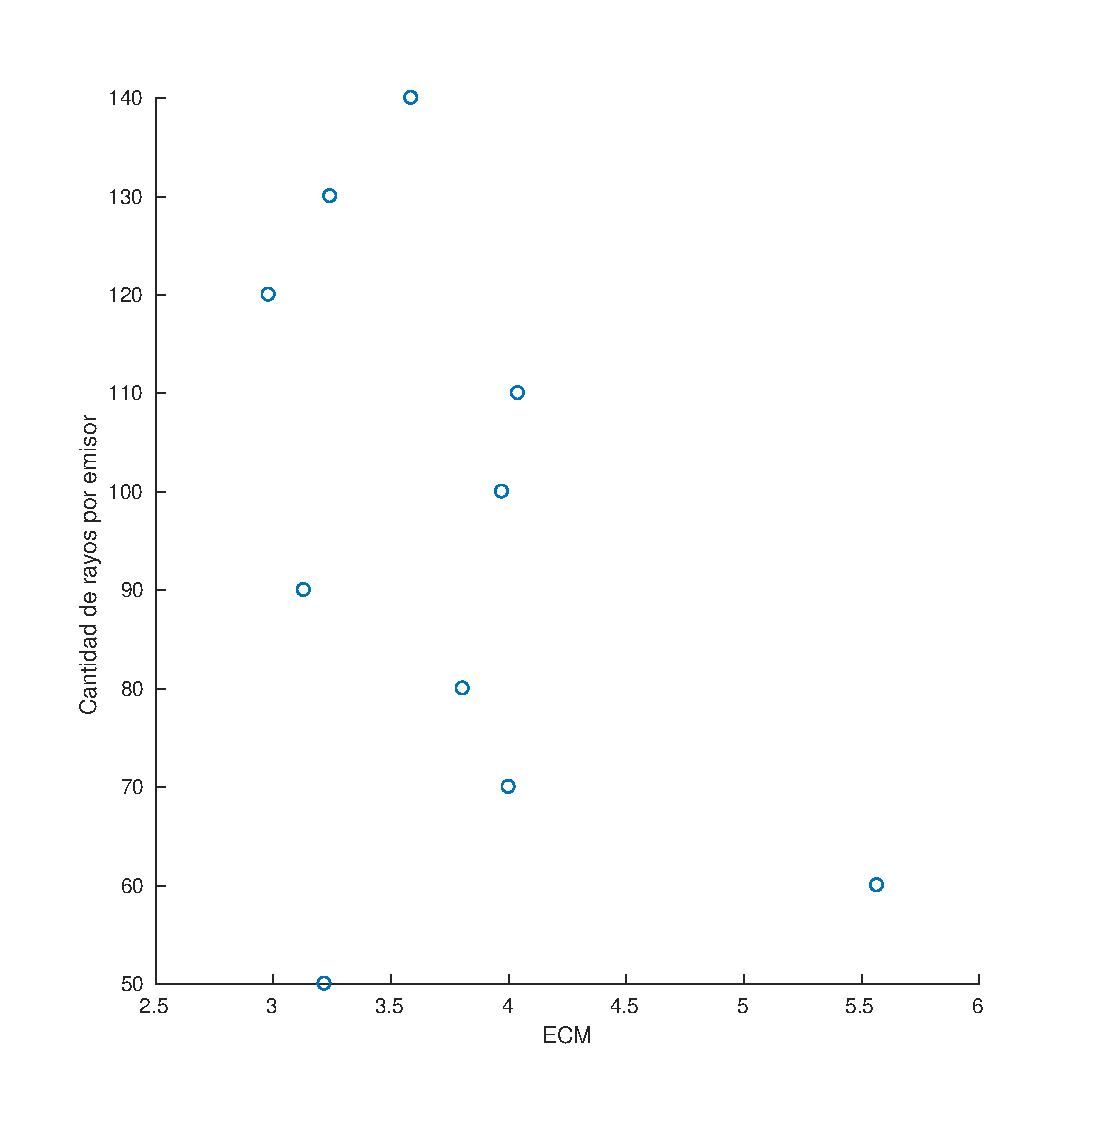
\includegraphics[width=0.7\textwidth]{img/cantrayos_ecm}
	\caption{ECM en funcion de la Cantidad de rayos con granularidad, cantidad de emisores y ruido fijos}
	\label{fig:cantrayos_eps}
\end{figure}

En este gráfico, esperamos que a medida que aumente la cantidad de informacion de la imagen, al incrementar el número de rayos por emisor, suba la calidad de la misma (baje el error cuadratico medio).  Sin embargo, en el gráfico podemos ver que la cantidad de rayos no aparenta tener ninguna relación con el ECM dentro de este rango (el programa no corre adecuadamente con menor cantidad de rayos por emisor porque se presentan celdas por las que no pasa ningun rayo con una alta probabilidad). Una posible explicación para ese fenomeno es  que la naturaleza aleatoria de la forma en que se construyen estos rayos lleva a que, cuando el número de rayos es suficiente para pasar por todos los pixeles de la imagen, ya se tiene suficiente información para que un incremento del número de rayos no cree una mejoría notable.

\begin{figure}[H]
	\centering	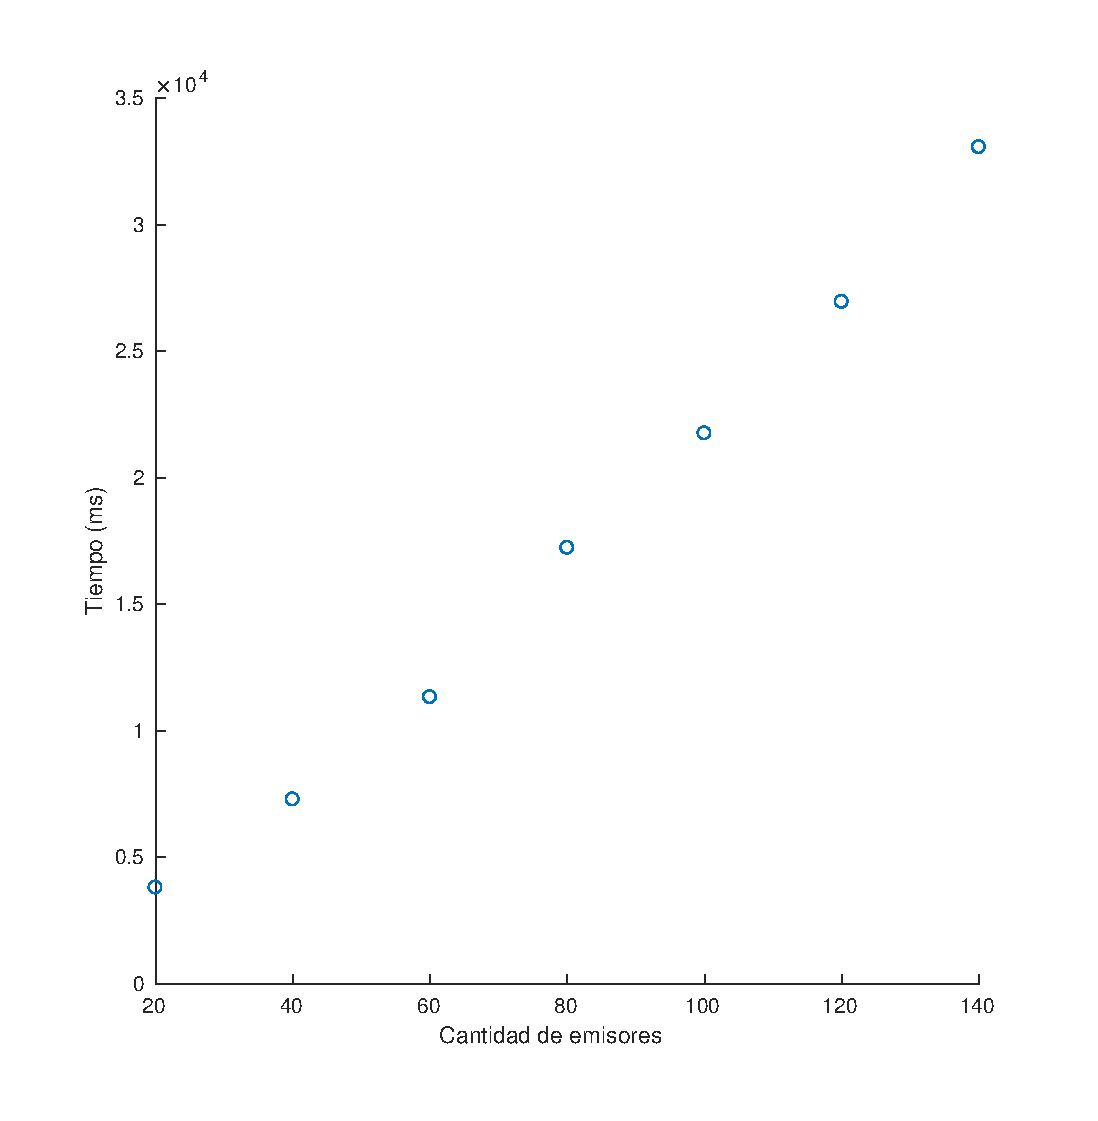
\includegraphics[width=0.7\textwidth]{img/emi_tiempo}
	\caption{Tiempo en funcion de la Cantidad de emisores con granularidad, cantidad de rayos por emisor y ruido fijos}
	\label{fig:emi_tiempo}
\end{figure}
\par Tal como se puede observar en este gr\'afico la cantidad de emisores de rayos afecta de manera directa en el tiempo de ejecuci\'on. Esto se debe a que nosotros mantuvimos fijos la cantidad de rayos por emisor, con lo cual, al aumentar
la cantidad de emisores estamos tambi\'en aumentando la cantidad total de rayos utilizados.

\begin{figure}[H]
	\centering	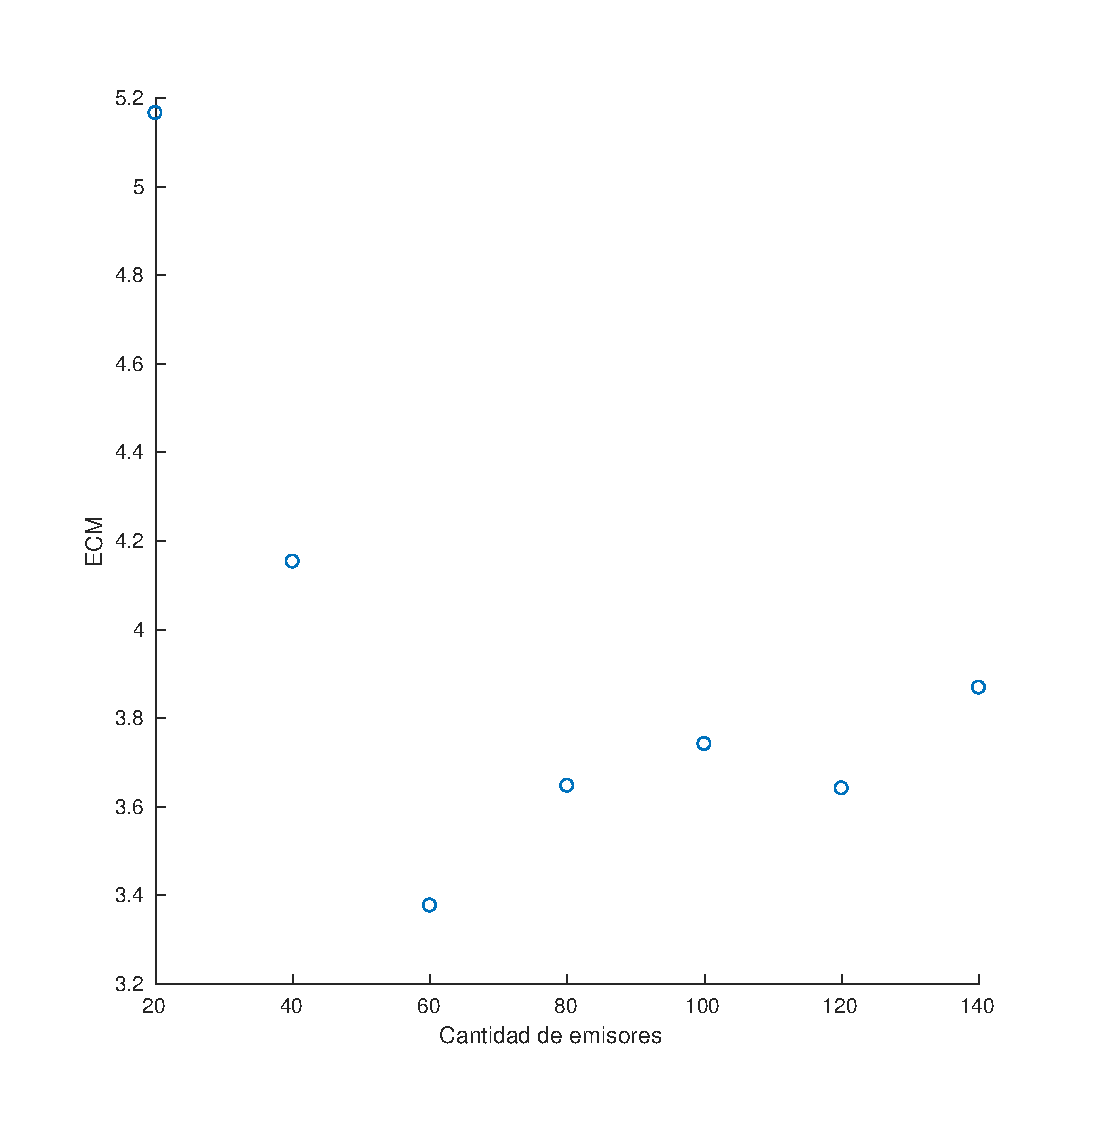
\includegraphics[width=0.7\textwidth]{img/emi_ecm}
	\caption{ECM en funcion de la Cantidad de emisores con granularidad, cantidad de rayos por emisor y ruido fijos}
	\label{fig:emi_ecm}
\end{figure}
De forma similar al ECM en funcion de la cantidad de rayos por emisor esperabamos que baje el error cuadratico a medida que aumenta el número de de emisores. Sin embargo, como se  puede ver que no hay una relación real entre la cantidad de emisores y el ECM dentro de este rango (el programa no corre con menor cantidad de emisores porque de hacerlo habría una muy alta probabilidad de que se presenten celdas por las que no pasa ningun rayo). La explicación para este fenómeno es la misma que en el caso previamente mencionado.

\begin{figure}[H]
	\centering	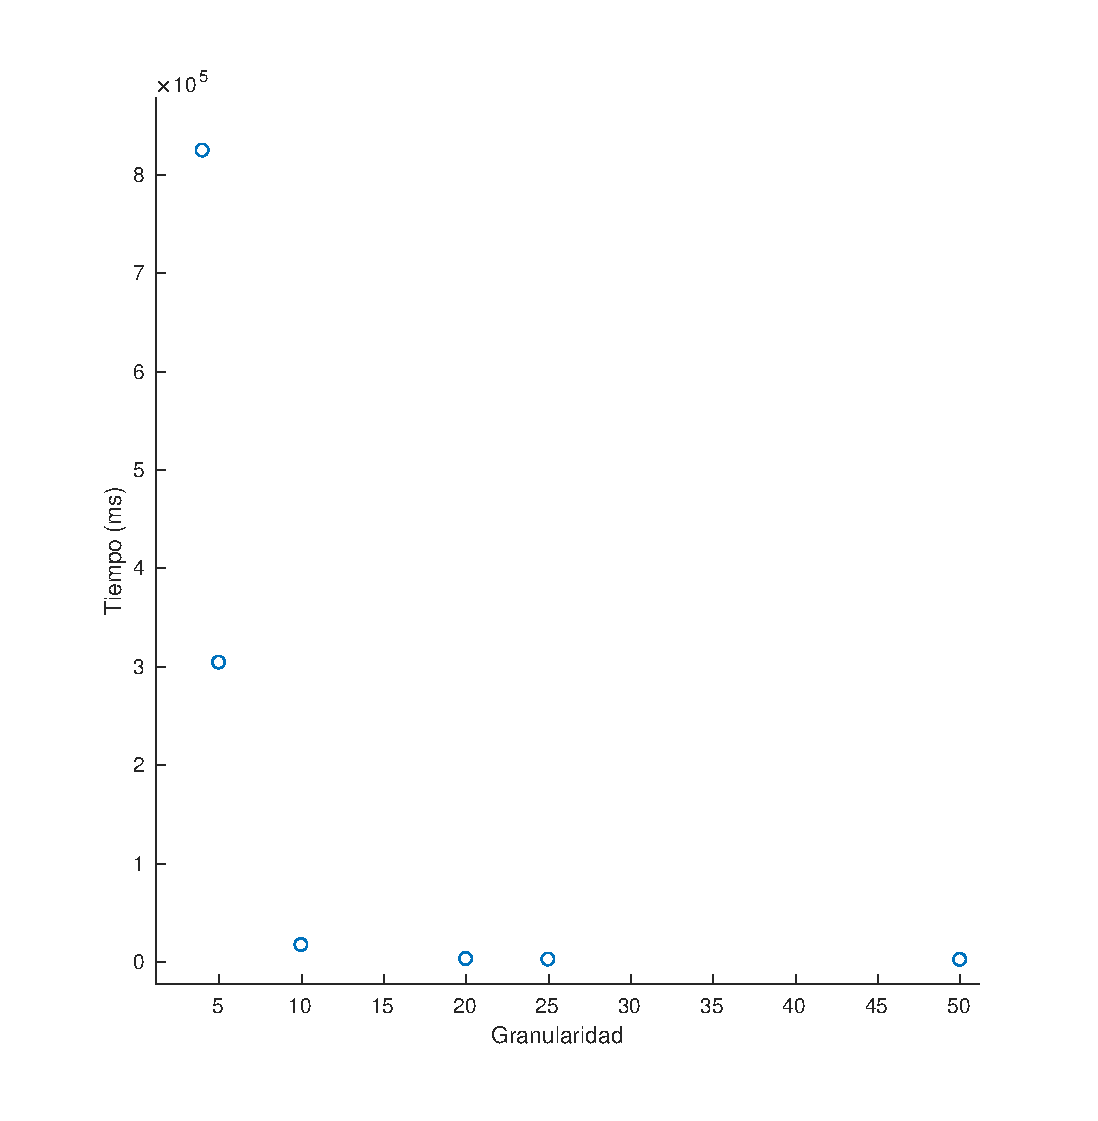
\includegraphics[width=0.7\textwidth]{img/granu_tiempo}
	\caption{Tiempo en funcion de la Granularidad con cantidad de rayos, cantidad de emisores y ruido fijos}
	\label{fig:granu_tiempo}
\end{figure}
\par A mayor granularidad, menor resulta el tiempo de ejecuci\'on debido a que casos de granularidad se reduce el tamaño de la matriz imagen.

\begin{figure}[H]
	\centering	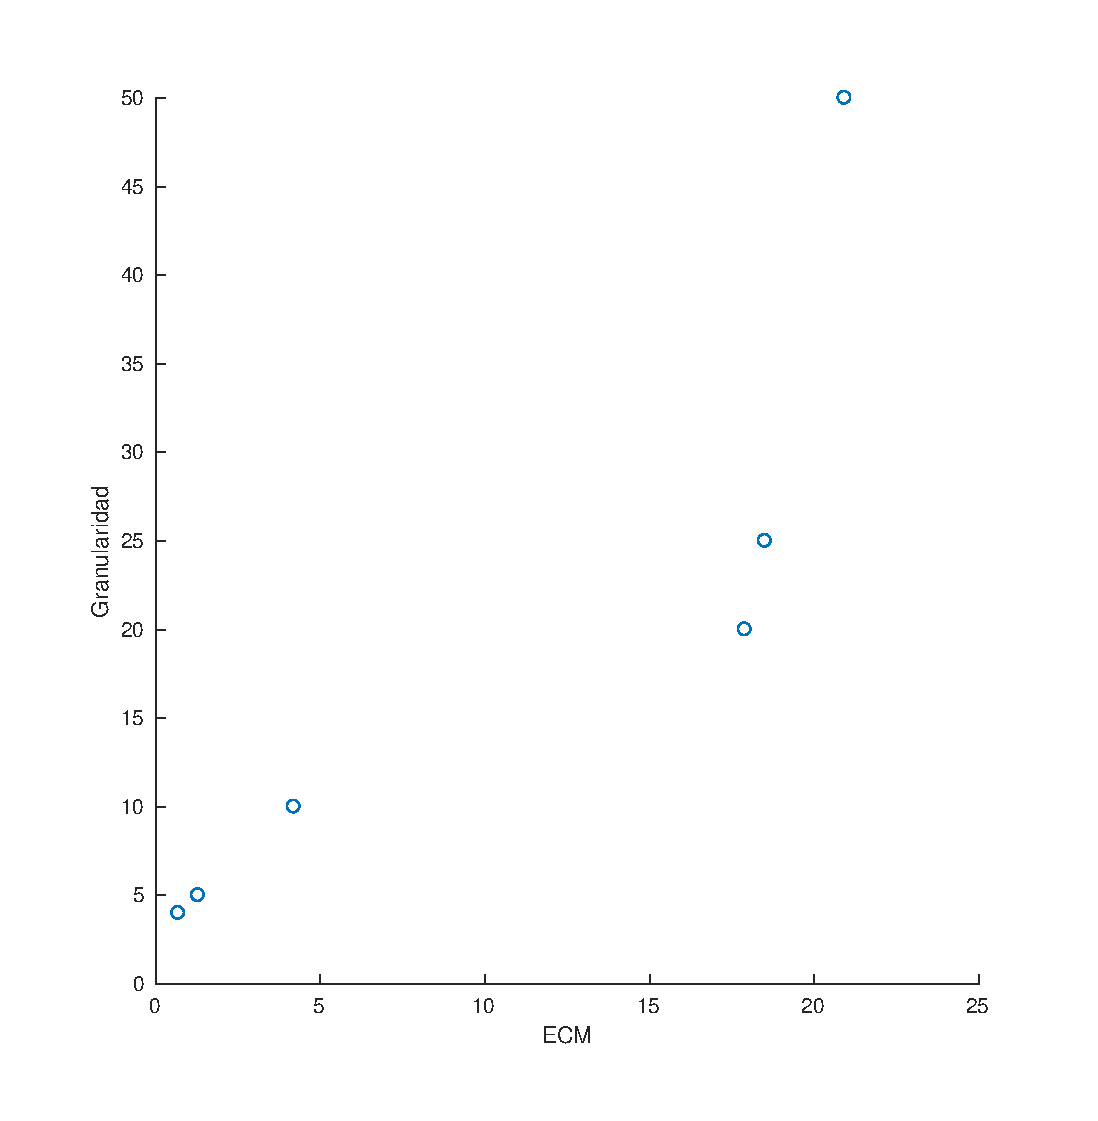
\includegraphics[width=0.7\textwidth]{img/granu_ecm}
	\caption{ECM en funcion de la Granularidad con cantidad de rayos, cantidad de emisores y ruido fijos}
	\label{fig:granu_ecm}
\end{figure}
Se espera que el error cuadrático medio aumente a medida que el número de celdas aumenta, ya que a mayor cantidad de celdas habrá un menor número de rayos que pase por cada una de ellas. Como se puede ver se confirma nuestra hipótesis y de hecho se puede ver que hay una relación lineal entre la granularidad y el ECM.

\begin{figure}[H]
	\centering	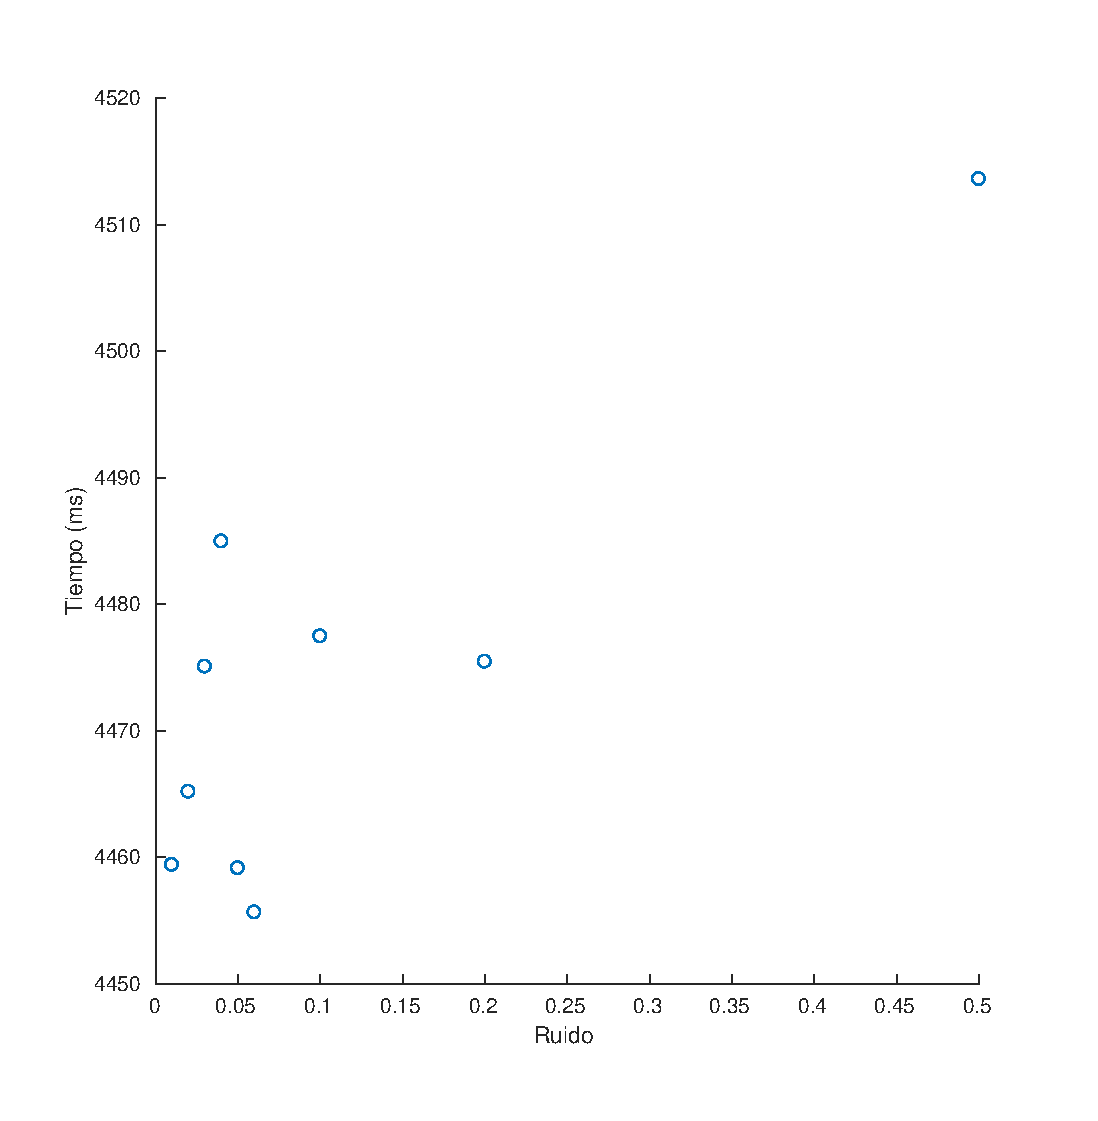
\includegraphics[width=0.7\textwidth]{img/ruido_tiempo}
	\caption{Tiempo en funcion del ruido con cantidad de rayos, cantidad de emisores y granularidad fijos}
	\label{fig:ruido_tiempo}
\end{figure}

\par Tal como esperabamos, el ruido que se le agrega a la imagen no afecta de manera significativa el tiempo de ejecuci\'on.

\begin{figure}[H]
	\centering	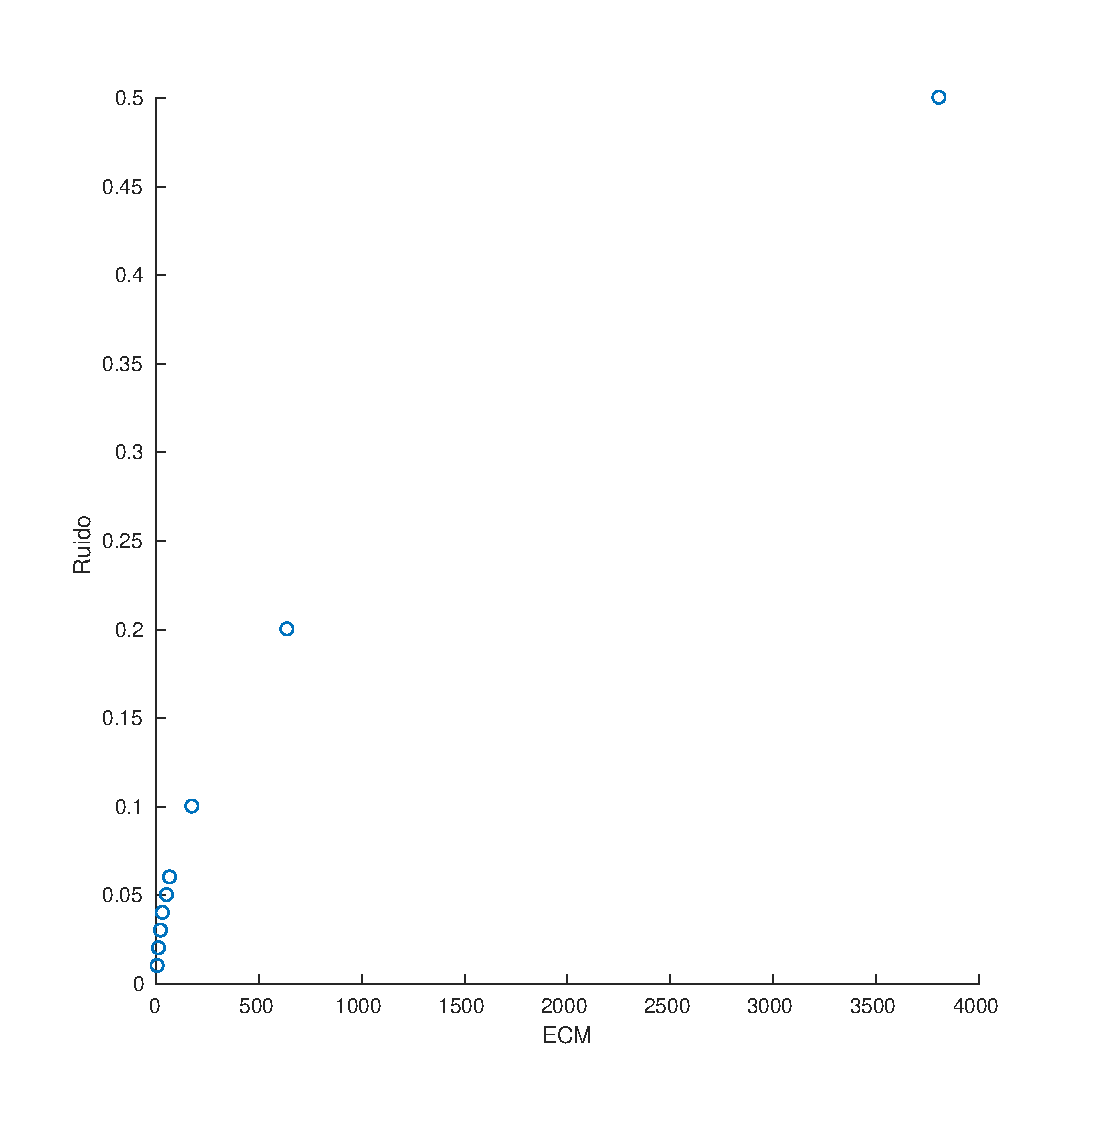
\includegraphics[width=0.7\textwidth]{img/ruido_ecm}
	\caption{ECM en funcion del ruido con cantidad de rayos, cantidad de emisores y granularidad fijos}
	\label{fig:ruido_ecm}
\end{figure}

